\chapter{Project Design - New}

This chapter outlines the design behind each component of the text classification model and the respected process each component may entail, several components will execute more than one step to achieve the desired result. The design is reflected within the final model and each component is broken down to display the functionality and theory within this project. In \autoref{section:FunctionalRequirements}, it is detailed there won’t be a GUI for the interaction and thus the design section relates to the inner workings of the model itself, that being: system architecture, logistics and theory.

\section{Classical vs Modern}

As originally intended, this project would have demonstrated two differing implementations of the same concept, one being of a classical nature implemented as a machine learning model and the other being a modern variation of the same approach, as previously mentioned this project experienced time management issues due to unexpected problems, to which resulted in only focusing on a traditional implementation within a modern model in attempt at a novel approach.

Classical NLP implementations can be described as:

\begin{figure}[H]
    \centering
    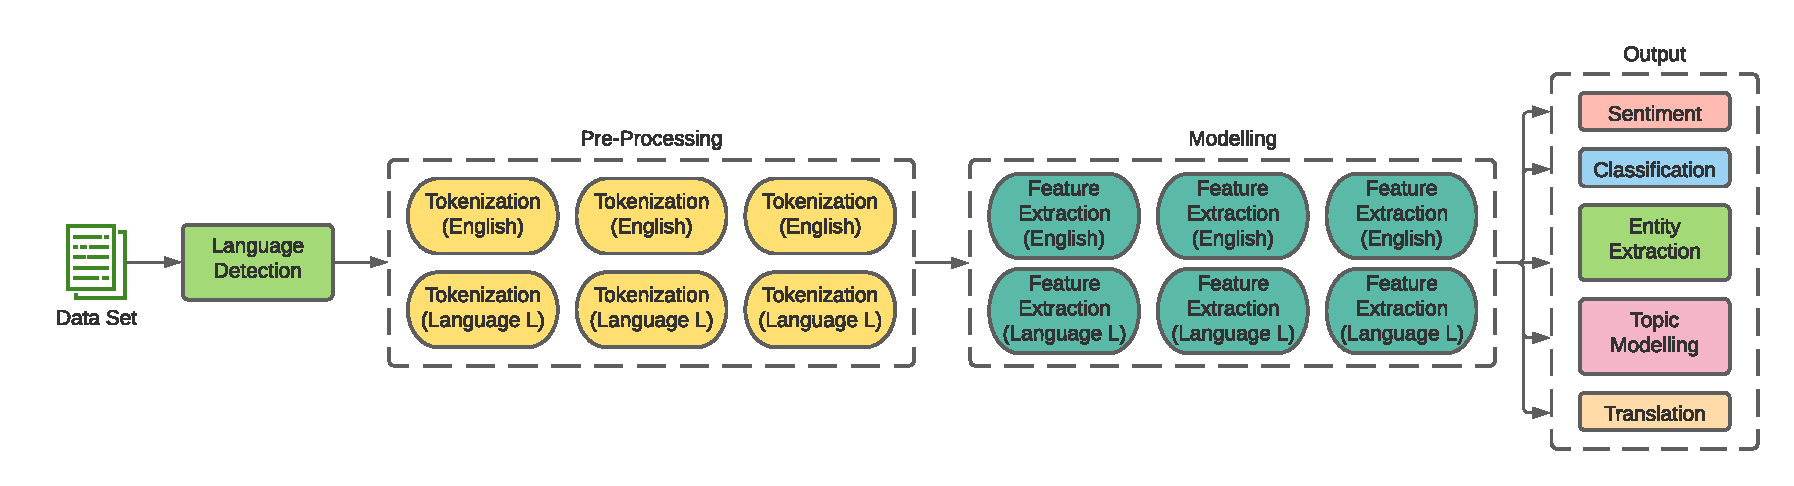
\includegraphics[width=\textwidth]{figures/chapter-5/ClassicalNLP.pdf}
    \caption[ClassicalNLP]{Classical NLP pipeline for text classification.
    \label{fig:ClassicalNLP}}
\end{figure}

Classical or "traditional" methods for corpus classification include: N-Grams, Hidden Markov Models using Markov Chains, Part-Of-Speech Tagging and Bag-Of-Words. Machine learning concepts can be classed as a “black-box” of functionality as the user does not necessarily see what is being executed within the hidden layers, a high-level abstraction for this project can be generalised into the following diagram:

\begin{figure}[H]
    \centering
    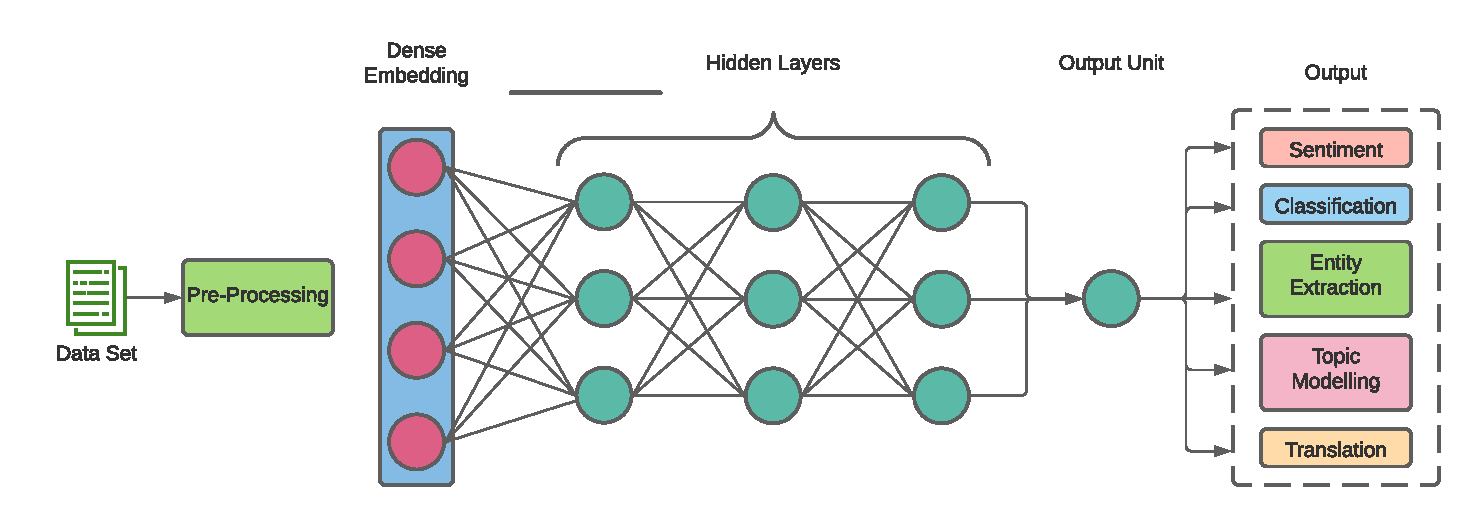
\includegraphics[width=\textwidth]{figures/chapter-5/MLNLP.pdf}
    \caption[MachineLearningNLP]{Machine Learning Model for an NLP pipeline for text classification.
    \label{fig:MLNLP}}
\end{figure}

\subsection{Model Approach --- Traditional}

The traditional implementation would have been designed based on word-embeddings within a 2D space where word vector values would be used alongside the Bag-Of-Words approach. The combination of Bag-Of-Words with a machine learning model to calculate a word’s vector based on its TF-IDF value would have been the start, such that:

\begin{equation}
    tf(t,d) = \frac{f_t, _d}{\sum{t \in_d} f _t {_`}, _d}
\end{equation}

Where the TF-IDF value is how often a lexeme occurs in a given corpus and would have also used the inverse TF-IDF value as the project model covers multiple datasets, such that:

\begin{equation}
    idf(t, D) = \log \frac{N}{|d \in D : t \in d|}
\end{equation}

Where the inverse TF-IDF value is represents how rare a word is in a given corpus.

\subsection{Limitations of Bag-Of-Words}

As there is a specific domain for this project, it is important to focus on the limitations for potential methods, CBOW models have demonstrated high training accuracy and is a relatively simple model to implement, it is naturally flexible as it can be trained on different datasets for a specific context; however, it does have disadvantages for classification and text prediction. Universities host students from different backgrounds and levels of education which can imply issues when training datasets, these issues can impact: the

\begin{itemize}
    \item \textbf{\textit{Vocabulary:}} Students may have varying output to describe the same context, this can create confusion for training.
    \item \textbf{\textit{Frequency:}} The frequency of a word may influence its power in a dataset.
    \item \textbf{\textit{Context:}} If students describe the same situation in a different way, some words may lose semantic meaning or be interpreted incorrectly, for example isolating neologisms, synonyms, colloquialism, polysemes, or semantic change.
\end{itemize}

\subsection{Model Approach --- Modern}

Modern or "contemporary" methods for corpus classification include: \ldots The modern implementation would have been based around Word2Vec implemented in a machine learning model for Sentiment Analysis which can be seen as a subcategory of text classification. The word2vec implementation would produce vector values for identified key words and plot them as such:

\begin{figure}[H]
    \centering
    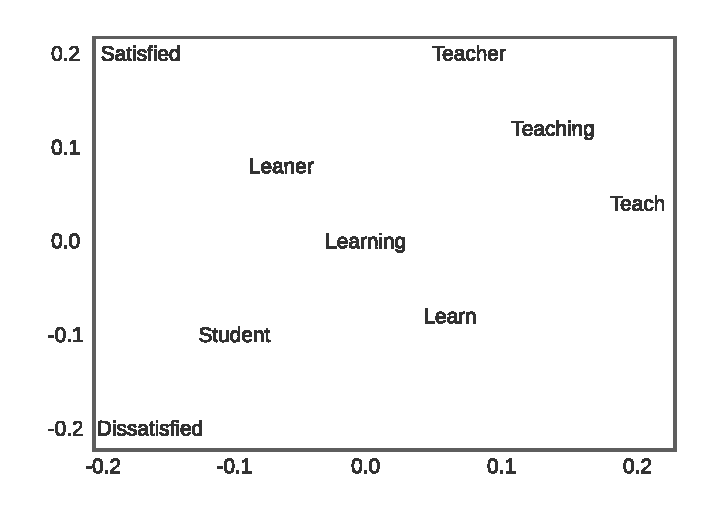
\includegraphics[width=\textwidth]{figures/chapter-5/Example-Word-Vector.pdf}
    \caption[ExampleWordVector]{Example of student satisfaction vector graph in 2d space.
    \label{fig:Example-Word-Vector}}
\end{figure}

\subsection{Word2Vec Skip-Gram}

Skip-gram rather than Continuous Bag-Of-Words (CBOW [which is the modern implementation of Bag-Of-Words]) as it yields better results with large datasets - such as student feedback - skip gram can also be context aware as it converts neighboring lexemes to vectors.

\begin{figure}[H]
    \centering
    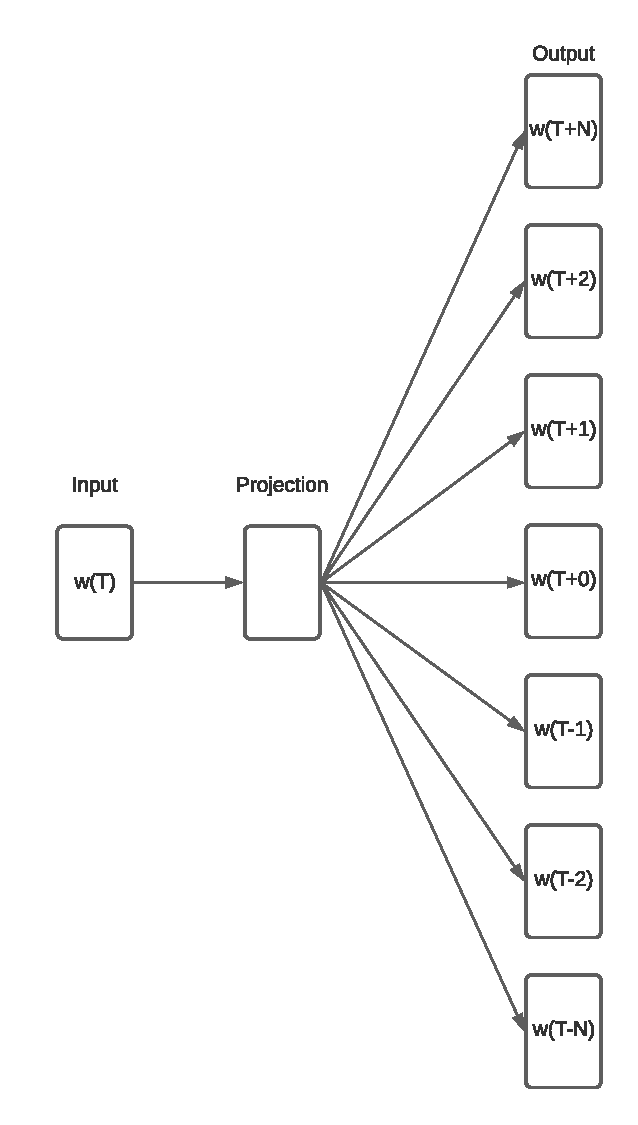
\includegraphics[width=0.49\textwidth]{figures/chapter-5/SkipGramModel.pdf}
    \caption[SkipGramModel]{Input flow of Skip-Gram model.
    \label{fig:SkipGramModel}}
\end{figure}

The skip-gram model can be seen as the inverse of the bag-of-words model as it attempts to vectorize neighboring words first to identify corpus context, whereas, bag-of-words takes each lexeme first, produces a vector sum and then categorises each word. \newpage

The Skip-Gram's network architecture is similar to the diagram displayed in \autoref{fig:MLNLP}, the diagram above is another level of abstraction as to how this project will make use of machine learning fundamentals.

\begin{figure}[H]
    \centering
    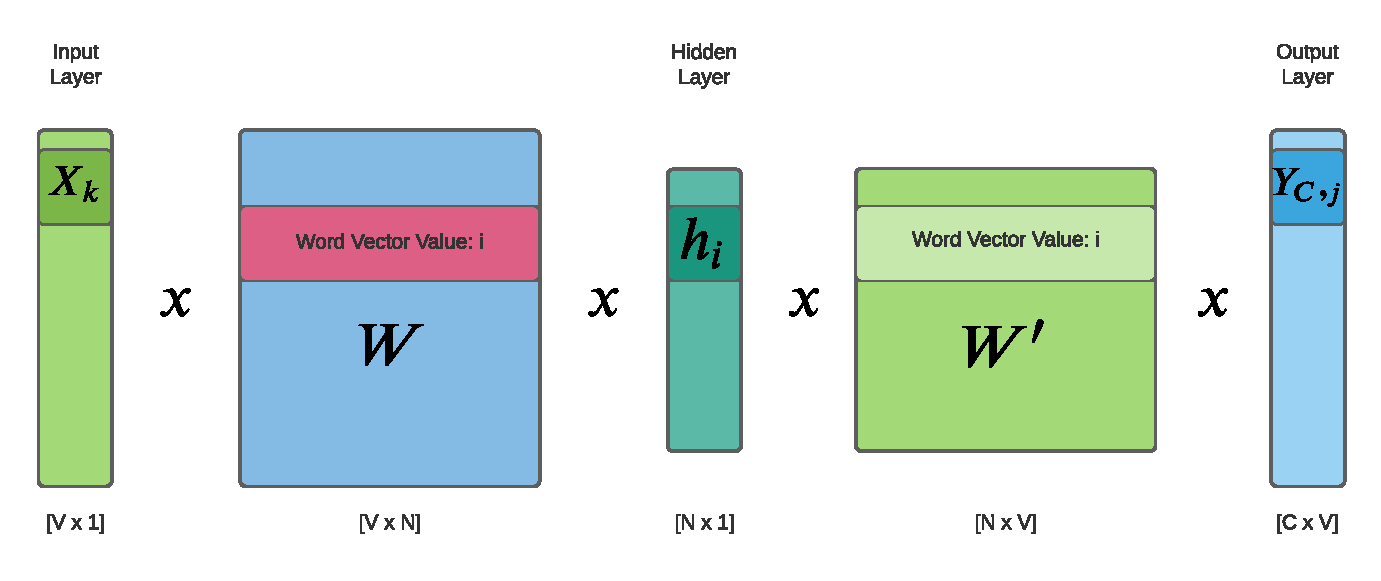
\includegraphics[width=\textwidth]{figures/chapter-5/SkipGramNetwork.pdf}
    \caption[SkipGramNetwork]{Skip-Gram implementation for Word2Vec network architecture.
    \label{fig:SkipGramNetwork}}
\end{figure}

\subsection{One-Hot Encoding}

Encoding each significant lexeme in a given dataset is helpful for the model to distinguish the level of importance, outlined as context, the diagram shown above in \autoref{fig:SkipGramModel} takes a 1D row vector as the input layer which allows for the model to acceptably one-hot encode each lexeme unit as a numeric value.

\begin{multicols}{2}
    \begin{equation*}
        "Teach" =
        \begin{bmatrix}
            0, & 0, & 0, & 0, & 1, & 0
        \end{bmatrix}
    \end{equation*}

    \begin{equation*}
        "Teaching" =
        \begin{bmatrix}
            0, & 0, & 0, & 0, & 1, & 0
        \end{bmatrix}
    \end{equation*}
\end{multicols}

This equates to differing versions of the same word (root + free or bound morpheme [affix]) to have the same influence when being parsed forward within the training model.

\subsection{Forward Propagation}

Once the corpus text is encoded as an acceptable 1D matrix, it can then be parsed to the first hidden layer's node:

\begin{equation}
    h = x^T W
\end{equation}
`x' represents the row vector, `h' can be taken as the column height ($[x]^T$ of the vector `W' where `h' is the `$k_{th}$' column.

\begin{equation}
    h = W_{(k,:)}^{T} \coloneqq v_{w_I}^{T}
\end{equation}
As each lexeme unit parses through the hidden layer nodes, the exit value needs to be calculated:

\begin{equation} \label{eq:u_cDefinition}
    u_{c} = W'^{T}h = W'^{T} W^{T}x
\end{equation}
For simplicity, $u_{c}$ will transpose each unit through the model in its entirety, however, the value(s) of $u_{c}$ cause performancy and memory issues in the model. Thus, \textbf{\textit{softmax}} will be used to slice the vector value of $u_{c}$ to [0,1].

\begin{equation*}
    y_{c} = Softmax(u)
\end{equation*}

\begin{equation}
    p(w_{c,_j} = w_{O,_c} | w_{I}) = y_{c,_j} = \frac{exp(u_{c_,j})}{\sum_{j' = 1}^{V} exp(u_{j'})}
\end{equation}
`x' represents the center word $w(T)$ of a vector where $W'$ will yield the softmax value of $u_{c}$, this ensures the vector of $w(T)$ will have exact values of input for `x', where:

\begin{multicols}{2}
    \begin{equation*}
        u_{c,_j} = u_{j} = {v'_{w_j}} ^ T \cdot h
    \end{equation*}

    \begin{equation}
        % TODO rewrite mathematically in set theory notation
        c=1 \ldots |C|
    \end{equation}
\end{multicols}
${v'_{w_j}}$ represents the exit vector for the $j^{th}$ lexeme unit in $w_{j}$ (the corpus vocabulary).

\subsection{Backward Propagation}

As stated below \autoref{eq:u_cDefinition}, the transposition of each unit $u_{c}$ is simple where node weight is not considered. To account for the weight of the model matrices $W$ and $W'$, the Stochastic Gradient Descent method is applied, which in turn will optimise the backward propagation of node errors; when training the model, errors are bound to occur, to which a loss function is needed to calculate each layers efficiency.

\begin{equation}
    \begin{split}
        Error (E) & = - \log \mathbb{P} (w_{O_,{_1}} , \ldots, w_{O_{,c}} | w_{I}) \\
                  & = - \log \prod_{c=1}^{C} \frac{exp(u_{c,j_{c}^{*}})}{\sum_{j'=1}^{V} exp(u_{j'})}  \\
                  & = - \sum_{c=1}^{C} u_{j_{c}^{*}} + C \cdot \log \sum_{j'=1} ^ {V} exp(u_{j'})
    \end{split}
\end{equation}
${j_{c}^{*}}$ represents the exit vector column's index within the vector's vocabulary. Once loss is calculated, the model can apply the \textbf{\textit{chain rule}} for weight error classification within $W$ and $W'$. This is achieved by obtaining the partial derivative of Error(E) of each exit node $u_{c,_j}$.

\begin{equation}
    \frac{\partial E}{\partial u_{c,_j}} = y_{c,_j} - t_{c,_j} \coloneqq e_{c,_j}
\end{equation}
$t_{c,_j}$ represents vector $u$'s \textbf{\textit{Ground Truth}}; [$t_{c,_j}$]'s state of hypothesis can be represented as the following definition:

\begin{equation}
    EI_j = \sum_{c=1}^{C} e_{c,_j} = \sum_{c=1}^{C} (y_{c,_j} - t_{c,_j}) = \frac{\partial E}{\partial u_{j}}
\end{equation}
$EI_{j}$ represents the \textbf{\textit{Row-Wise Sum}} as a column vector in attempt to account for word context errors for $w(T)$; \textbf{\textit{backpropagation}} can then occur by obtaining the partial derivative of Error(E) within matrix $W'$.

\begin{equation} \label{}
    \begin{split}
        \frac{\partial E}{\partial w'_{ij}} & = \sum_{c=1}^{C} \frac{\partial E}{\partial u_{c_{,j}}} \cdot \frac{\partial u_{c_{,j}}}{\partial w'_{i_{,j}}} \\
                                            & = \sum_{c=1}^{C} (y_{c,_j} - t_{c,_j}) \\
                                            & = EI_{j} \cdot h_{i}
    \end{split}
\end{equation}
When backpropagation occurs, the Stochastic Gradient Descent is redefined in terms of the matrix $W'$:

\begin{equation}
    w'^{(new)}_{i,j} = w'^{(old)}_{i,j} - \eta \cdot EI_{j} \cdot h_{i}
\end{equation}
$\eta$ represents the model's training (learning). Once the learning rate has been established, the model can update the distribution of errors between the model layers, particularly between unit input and the hidden layer whereby the partial derivative is weighted against an error from a hidden layer. This can be calculated with:

\begin{equation}
    \begin{split}
        \frac{\partial E}{\partial h_{i}} & = \sum_{j=1}^{V} \frac{\partial E}{\partial u_{j}} \cdot \frac{\partial u_{j}}{\partial h_{i}} \\
                                          & = \sum_{j=1}^{V} EI_{j} \cdot w'_{ij}
    \end{split}
\end{equation}
As errors are calculated between the input layer and the hidden layer accounting for error weight, it is possible to calculate the weighted loss of matrix $W$ by taking the partial derivatives of Error(E) against the partial derivative of an index within matrix $W$, as such:

\begin{equation} \label{}
    \begin{split}
        \frac{\partial E}{\partial W_{ki}} & = \frac{\partial E}{\partial h_{i}} \cdot \frac{\partial h_{i}}{\partial w_{ki}} \\
                                           & = \sum_{j=1}^{V} EI_{j} \cdot w'_{ij} \cdot x_{k}
    \end{split}
\end{equation}
The weight of the Stochastic Gradient Descent is redefined in terms of the matrix $W$:


\begin{equation}
    w^{(new)}_{i,j} = w^{(old)}_{i,j} - \eta \cdot \sum_{j=1}^{V} EI_{j} \cdot w'_{ij} \cdot x_{j}
\end{equation}
The fundamental functionality has been outlined in theory but in practice will be enough to train the given Skip-Gram Network in \autoref{fig:SkipGramNetwork}.

% TODO rewrite mathematical improvements to include future work.
% \begin{equation}
%     \textbf{\textit{score}}(w_{a}, w_{b}) = \frac{\textbf{\textit{count}}(w_{a}w_{b}) - \delta}{\textbf{\textit{count}}(w_{a}) \times \textbf{\textit{count}}(w_{b})}
% \end{equation}

% \begin{equation}
%     P(w_{i}) = 1 - \sqrt{\frac{t}{f(w_{i})}}
% \end{equation}

% \begin{equation}
%     \log p(w | w_{i}) = \log \sigma ({v'}_{w}^{T} v_{w_{I}}) + \sum_{i=k}^{K} E_{w_{i}P_{n}(w)} \left [ \log \sigma (-{v'}_{w}^{T} v_{w_{I}}) \right ]
% \end{equation}

\section{Planning the ML Model Design}

Initial prototyping of the machine learning model for a new amalgamation of NLP techniques helped to indicate what the best route of development could be, the planning stage piggybacked off existing work flowchart diagrams in-order to apply the most appropriate method and technique combination. The sequence flowchart is as follows:

\begin{figure}[H]
    \centering
    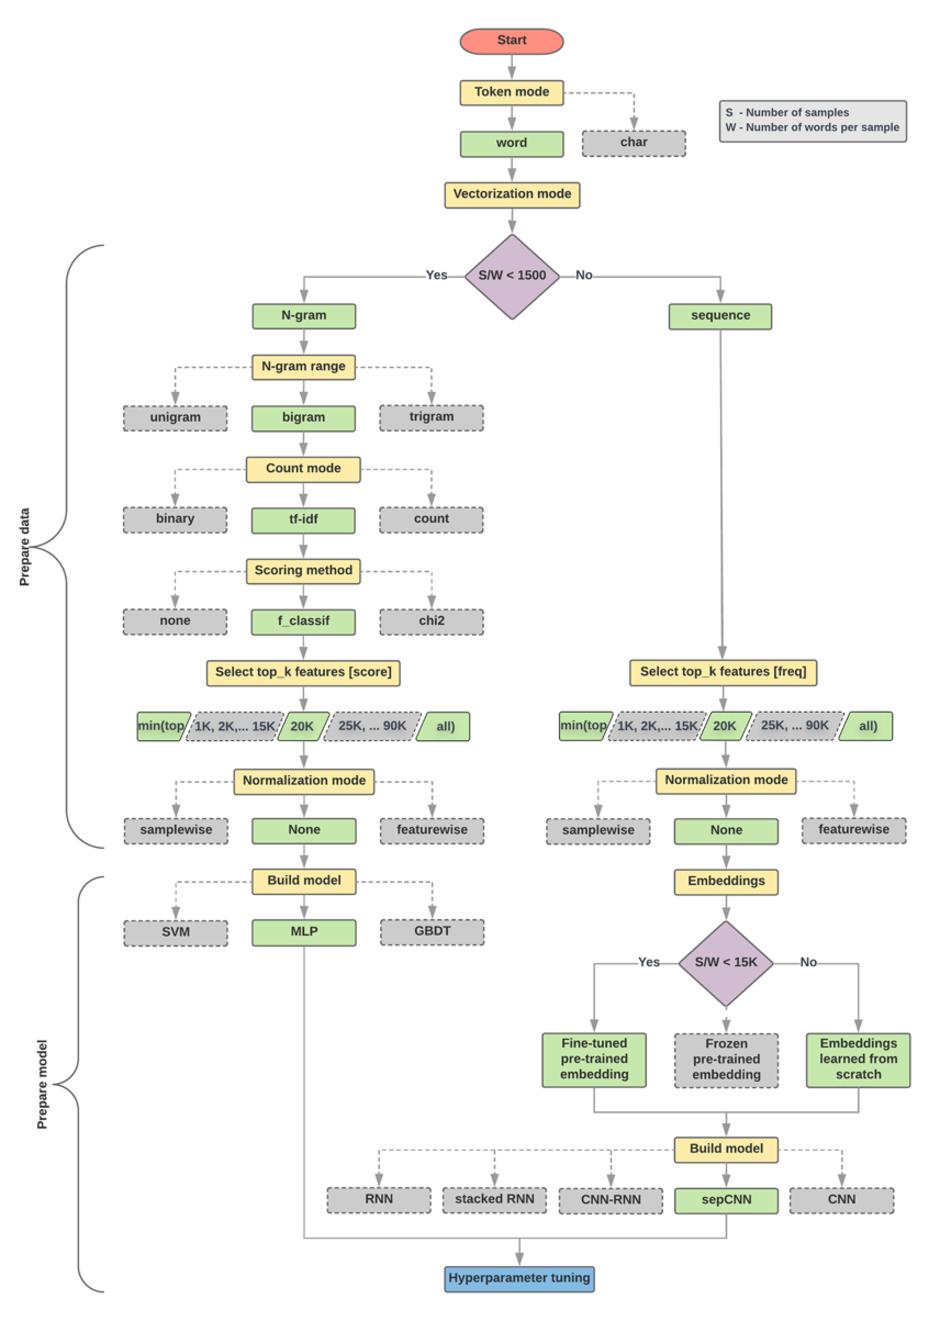
\includegraphics[width=\textwidth]{figures/chapter-5/GooglePlan.pdf}
    \caption[GooglePlan]{Text Classification Flowchart \parencite{google2021TCF}.
    \label{fig:GooglePlan}}
\end{figure}

\section{Supervision}

The development of the project model is based on a supervised approach due to the datasets located, it was most appropriate to use a supervised approach due to the datasets having no labels or lexical categories to train the model on; the model has user input to account for missing labels on data which have been manually and algorithmically added. The supervision for this project can be represented as the following diagram:

\begin{figure}[H]
    \centering
    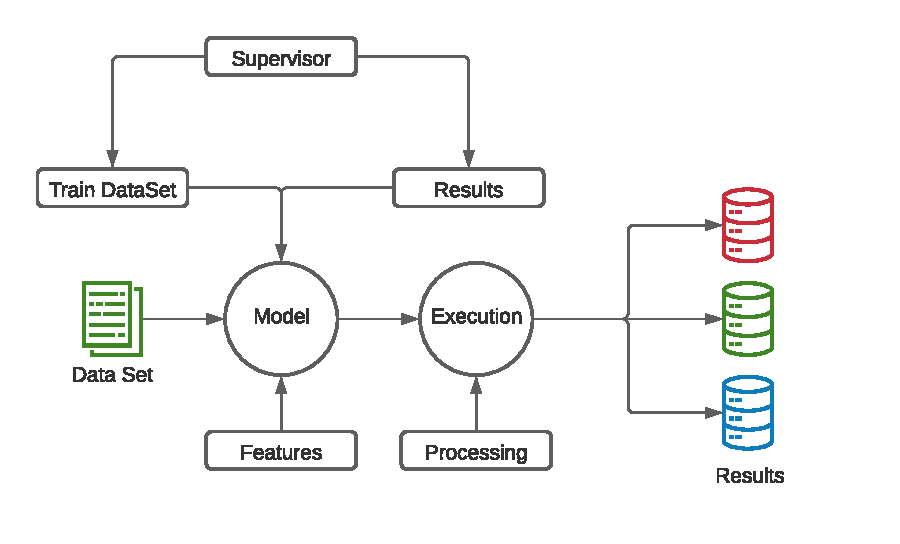
\includegraphics[width=\textwidth]{figures/chapter-5/SupervisedLearningChart.pdf}
    \caption[SupervisedLearning]{Sequence control for Supervised learning.
    \label{fig:SupervisedLearningChart}}
\end{figure}

\section{Pipeline Design}

\begin{figure}[H]
    \centering
    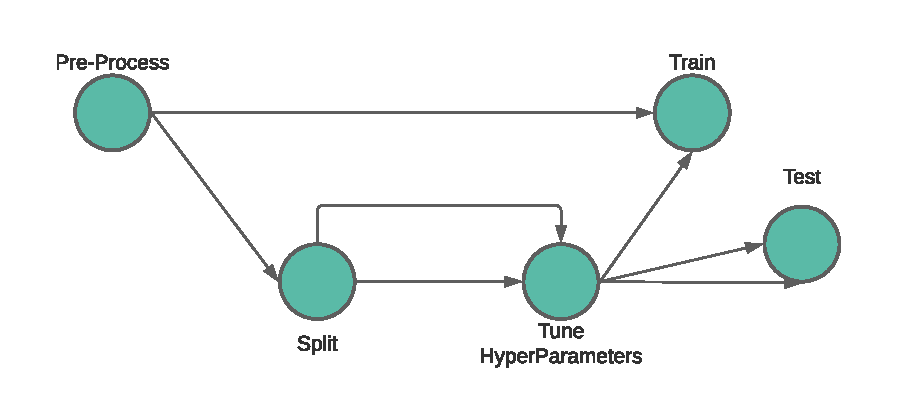
\includegraphics[width=\textwidth]{figures/chapter-5/Pipeline.pdf}
    \caption[MLTCPipeline]{Pipeline for model classification.
    \label{fig:MLTCPipeline}}
\end{figure}

There are five main steps for a text classification pipeline:

\begin{enumerate}
    \item \textbf{\textit{Pre-processing}}: prepare the raw dataset to be trained.
    \item \textbf{\textit{Splitting}}: split the processed dataset to be trained and validated.
    \item \textbf{\textit{Tuning}}: identity valuable parameters within trained data.
    \item \textbf{\textit{Training}}: train the current iteration of the model with updated hyper-parameters.
    \item \textbf{\textit{Testing}}: test and collect statistics for analysis to make further predictions.
\end{enumerate}

\section{Data Preparing and Pre---processing}